\documentclass{article}\usepackage[]{graphicx}\usepackage[]{color}
%% maxwidth is the original width if it is less than linewidth
%% otherwise use linewidth (to make sure the graphics do not exceed the margin)
\makeatletter
\def\maxwidth{ %
  \ifdim\Gin@nat@width>\linewidth
    \linewidth
  \else
    \Gin@nat@width
  \fi
}
\makeatother

\definecolor{fgcolor}{rgb}{0.345, 0.345, 0.345}
\newcommand{\hlnum}[1]{\textcolor[rgb]{0.686,0.059,0.569}{#1}}%
\newcommand{\hlstr}[1]{\textcolor[rgb]{0.192,0.494,0.8}{#1}}%
\newcommand{\hlcom}[1]{\textcolor[rgb]{0.678,0.584,0.686}{\textit{#1}}}%
\newcommand{\hlopt}[1]{\textcolor[rgb]{0,0,0}{#1}}%
\newcommand{\hlstd}[1]{\textcolor[rgb]{0.345,0.345,0.345}{#1}}%
\newcommand{\hlkwa}[1]{\textcolor[rgb]{0.161,0.373,0.58}{\textbf{#1}}}%
\newcommand{\hlkwb}[1]{\textcolor[rgb]{0.69,0.353,0.396}{#1}}%
\newcommand{\hlkwc}[1]{\textcolor[rgb]{0.333,0.667,0.333}{#1}}%
\newcommand{\hlkwd}[1]{\textcolor[rgb]{0.737,0.353,0.396}{\textbf{#1}}}%
\let\hlipl\hlkwb

\usepackage{framed}
\makeatletter
\newenvironment{kframe}{%
 \def\at@end@of@kframe{}%
 \ifinner\ifhmode%
  \def\at@end@of@kframe{\end{minipage}}%
  \begin{minipage}{\columnwidth}%
 \fi\fi%
 \def\FrameCommand##1{\hskip\@totalleftmargin \hskip-\fboxsep
 \colorbox{shadecolor}{##1}\hskip-\fboxsep
     % There is no \\@totalrightmargin, so:
     \hskip-\linewidth \hskip-\@totalleftmargin \hskip\columnwidth}%
 \MakeFramed {\advance\hsize-\width
   \@totalleftmargin\z@ \linewidth\hsize
   \@setminipage}}%
 {\par\unskip\endMakeFramed%
 \at@end@of@kframe}
\makeatother

\definecolor{shadecolor}{rgb}{.97, .97, .97}
\definecolor{messagecolor}{rgb}{0, 0, 0}
\definecolor{warningcolor}{rgb}{1, 0, 1}
\definecolor{errorcolor}{rgb}{1, 0, 0}
\newenvironment{knitrout}{}{} % an empty environment to be redefined in TeX

\usepackage{alltt}
\usepackage{amsmath,underscore,graphicx}
\usepackage[margin=1in]{geometry}
\graphicspath{{./figure/}}
\newcommand{\mic}{$ft > 4 \times MIC$}
\IfFileExists{upquote.sty}{\usepackage{upquote}}{}
\begin{document}




% Outline:
% 1. Introduction
% 2. Methods
%  - PK model (two-compartment)
%  - PD summaries (T>MIC)
%  - Statistical model (Bayesian NLR); prior and where it comes from
%  - Approximate intervals for MIC statistic
%  - Evaluating quality of approximate intervals
%  3. Results; summary of CI quality
%  4. Examples
%  5. Discussion/conclusion; potential extensions
%  - statistical [covariates, different types of models]
%  - applications)
% Extensions
% Conclusions

%\section{Introduction}
%\begin{itemize}
%\item Goal is to facilitate real-time herapeutic drug monitoring (TDM); translational research.
%\item PK predictions often not reported with uncertainty; cite literature.
%\item Need to quantify uncertianty in real time, but it's difficult.
%\item incorporate objective prior information
%\item We created a web app and suite of methods that accomplish this.
%\end{itemize}

%[need references]
Adverse medical consequences can arise from both antibiotic underdosing and overdosing of hospitalized patients. In the former case, patients receive an insufficient amount of antibiotic to effectively combat infection. In the latter, an overabundance of antibiotic may increase the risk of toxicity. However, the pharmacokinetics and pharmacodynamics of common antibiotics, such as piperacillin and ciprofloxacin, can exhibit substantial variability among hospitalized patients due to patient characteristics (e.g., body mass) or complications (e.g., organ failure) **. As a result, simple algorithmic dosing strategies (e.g., based on creatinine alone) can fail to ensure an appropriate level of antibiotic exposure.\\
%**\cite{Shotwell2015, Shotwell2016} - need to sort out bibtex

For an individual patient, pharmacokinetic uncertianty can be reduced by measuring drug concentration in the blood over time. These data can be used to estimate current and past drug exposure, predict future drug exposure under alternative dosing strategies, and adjust the dose accordingly. The methods and software presented herein were designed to implement this process using prior information about pharmacokinetic heterogeneity in the target population and, if available for the individual, measurments of drug concentration in the blood over time. In order to impact clinical decision making, these tasks must be accomplished in real-time and account for (often substantial) statistical uncertainty.\\

We implement Bayesian methods using pharmacokinetic data from a prior study [cite] to provide posterior estimates of individual target attainment, measured as the fraction of the dosing period spent above a specified blood concentration threshold; usually a multiple of a minimum inhibitory concentration (MIC). The minimum inhibitory concentration is the amount of the drug required to suppress the offending microorganism. This particular summary of target attainment (denoted $T>k$MIC, where $k$ is positive) is useful for antibiotics that have time-dependent effectiveness. Other summaries, such as the peak concentration, may be useful for antibiotics with concentration-dependent effectiveness. Due to significant pharmacokinetic heterogeneity, measures of statistical uncertainty about $T>k$MIC are critical for understanding response to treatment at the patient-specific level, and for clinical decision-making. We summarize this statistical uncertainty by computing and presenting 95\% credible intervals for patient-specific estiamtes of $T>k$MIC. However, in order for these methods to be practicable, it is necessary that computation can occur in real time. Due to the computational intensity of exact methods (e.g., Markov chain Monte Carlo), we sought to identify statistical approximations that are both accurate with regard to quantification of statistical uncertainty (i.e., the effective level of the approximate credible interval closely matches the nominal level, 95\%) while also being computationally feasible to implement with no significant delay (e.g., via a web application). We accomplish this by using a serie of statistical approximations paired with a web application that renders these techniques accessible to, for example, a practicing physician. We present assessments of the accuracy and computational efficiency for this approach.

% [MSS note: I think this need to be in the last paragraph of the introduction] The aim of this work is to facilitate accurate, real-time therapeutic drug monitoring (TDM).




\section{Methods}
\subsection{Two-compartment model}
The two-compartment pharmacokinetic model is expressed as a system of two ordinary differential equations as follows, where $m_1$ and $m_2$ are the masses of drug in the central and peripheral compartments, respectively.

\begin{align}
\frac{dm_1}{dt} &= -k_{10}m_1 - k_{12}m_1 + k_{21}m_2 + k_R \nonumber \\
\frac{dm_2}{dt} &= \phantom{-k_{10}m_1} + k_{12}m_1 - k_{21}m_2 \nonumber
\end{align}

The concentration of drug in the central compartment is given by $c_1 = m_1/v_1$, where $v_1$ is the volume of the central compartment. The parameters $k_{10}$, $k_{12}$, $k_{21}$, and $k_R$ are described in Table \ref{tab:pkpars}

\begin{table}
\begin{tabular}{lll} \hline
Parameter & Units & Description \\ \hline
$k_{10}$ & h$^{-1}$ & Elimination rate from central compartment\\
$k_{12}$ & h$^{-1}$ & Distribution rate from central to peripheral compartment\\
$k_{21}$ & h$^{-1}$ & Distribution rate from peripheral to central compartment\\
$k_R$  & g$\cdot$h$^{-1}$ & Infusion rate into central compartment\\
$v_1$  & L & Volume of central compartment\\
\hline
\end{tabular}
\caption{Two-compartment model parameter units (SI) and descriptions. \label{tab:pkpars}}
\end{table}

% Is "dosing window" the appropriate terminology here
% alternative: observation period
To assess patient response to treatment by measuring {\it target attainment}, defined in this context to be the fraction of dosing window for which the concentration of piperacillin in the bloodstream is 64$\mu$g/mL: four times the minimum inhibitory concentration (MIC) for piperacillin. We denote this statistic as \mic. Dosing for a patient needs to be enough that the concentration in the blood remains above the necessary threshold for suppression of the offending microorganism, yet not so high as to increase the risk of adverse side effects including toxicity. Typically, a multiple of the minimum inhibitory concentration is used for such measurements, since drug concentration is attenuated in muscle tissue relative to the bloodstream. \\

% Insert link to next section for concentration-time curve. I mention it in this calculation but it's derived from the Bayesian model below.
We measure \mic by calculating a simple proportion of the time during the dosing window above 64$\mu$g/mL. By default, the method considers the conclusion of the full dosing window to be 12 hours after the end of the final infusion. If implementing this method with other medications, the limit of the dosing window may need to be altered based on drug-specific properties such as the rate of elimination. We use a bisection root-finding method to identify the times at which the patient's concentration-time curve crosses 64$\mu$g/mL. Drug concentration increases if and only if the drug is actively being infused intravenously. Once the IV is removed, the drug concentration can only decrease. Thus, the adjacent time points at which one infusion ends and the next begins (and vice versa) are used as endpoints in the bisection process.\\


% Is this more relevant here or in the Bayesian model section?
% Is the 50% threshold generally a target? Or was that just for the prior study/other paper?
Time 0 is taken to be the time of first drug infusion. This assumes that the concentration of drug in the patient's body is 0$\mu$g/mL at time 0. A specific pharmacodynamic target is usually outlined. In this case where we are considering piperacillin, the target is \mic $> 0.5$, or at least half of the dosing window is spent above the desired threshold.

% There are specific criteria for spending a certain amount of time above the threshold, are there accepted criteria for toxicity thresholds? (defined either by time or concentration or a combination between the two) - is this something we need to address?



\subsection{Bayes prediction model} % statistical model
% Insert label to connect to previous section where I mention the concentration time curve
Concentration measurements are modeled using a nonlinear regression method with additive error as follows:
\begin{displaymath}
c_{ij} = \eta_i(t_{ij}, \theta_i) + \epsilon_{ij}
\end{displaymath}
\noindent In this expression, $c_{ij}$ is the measured concentration for subject $i = 1 \ldots n$ at time $t_{ij}$ for $j = 1 \ldots m_i$, $\eta_i(t_{ij}, \theta_i)$ is the two-compartment model solution for subject $i$ at time $t_{ij}$ given parameters $\theta_i = [k_{10i}, k_{12i}, k_{21i}, v_{1i}]$, and $\epsilon_{ij}$ represents i.i.d. random error with mean zero. By specifying the random error density function, say $f(\epsilon_{ij}, \sigma)$, the subject-specific likelihood function is
\begin{displaymath}
L_i(\theta_i, \sigma) = \prod_{j=1}^{m_i} f(c_{ij} - \eta_i(t_{ij}, \theta_i), \sigma).
\end{displaymath}
\noindent Thus, given a prior distribution $\pi_0(\theta_i)$, the subject-specific posterior is proportional to $\pi_i(\theta_i, \sigma) \propto \pi_0(\theta_i,\sigma)L_i(\theta_i,\sigma)$.

In the current context, $f$ is taken as the normal density function with mean zero and standard deviation $\sigma$, and the prior distribution is generated to satisfy the following:
\begin{align}
[\log \theta_i] &\sim N_4(\mu_0, \Sigma_0) \\
[\log \sigma] &\sim N_1(m_0, s_0)
\end{align}
\noindent where $N_4(\mu_0, \Sigma_0)$ represents the 4-variate normal distribution with mean $\mu_0$ and covariance matrix $\Sigma_0$ for the pharmacokinetic parameters, and $N_1(m_0, s_0)$ represents the univariate normal distribution with mean $m_0$ and variance $s_0$. The prior distribution for the PK parameters represents our prior knowledge about the PK heterogeneity for a particular drug in a target population. Thus, the values of the prior hyperparameters should be carefully selected for the task at hand. In the current context, and by default, the hyperparameters are specified to correspond with estimates that arose from a study of piperacillin pharmacokinetics in a hospitalized, critically ill population. The particular values are listed in an appendix.

Due to the nonlinearity of the two-compartment model, the posterior distribution does not take a familiar form, and posterior summaries must be approximated. In particular, we sought to compute 95\% credible bands for subject-specific concentration-time curves, and for a specific summary of the curve (\mic). Monte Carlo techniques are often used to approximate these quantities. However, because these posterior summaries are presented in a web application in real time, we sought alternatives that were less computationally intensive and deterministic. Implementation of Laplace and delta method approximations allow for rapid computation of posterior estimates.

We consider several possible types of intervals for \mic: logit-transformed, probit-transformed, and untransformed intervals. Logit- and probit-transformed intervals restrict the computed confidence interval boundaries to be between 0 and 1. Untransformed intervals can yield bounds above 1, in which case the upper confidence limit is truncated at 1. The untransformed 95\% credible interval is computed as $\hat{\theta} \pm z_{0.975} SE(\hat{\theta})$. Gradients for the transformed intervals are computed using the delta method.


\subsubsection{Laplace approximation}
We first considered a method that makes use of two approximations. The first is a Laplace approximation to the subject-specific posterior density, and the second is a first order Taylor approximation of the target summary (i.e., the `delta method'). The Laplace approximation is given as follows
$$\pi_i(\log \theta_i, \log \sigma) \approx N([\log \hat{\theta_i},\log \hat{\sigma}], [-H]^{-1})$$
\noindent where $[\log \hat{\theta_i},\log \hat{\sigma}]$ is the posterior mode and $H_{\hat{\theta_i}}$ is the posterior Hessian with respect to $[\log \theta_i, \log \sigma]$ evaluated at the posterior mode. The second approximation makes use of the delta method, such that a posterior functional $h(\log \theta_i)$ has an approximate normal distribution. In the present context, $h(\log \theta_i)$ represents the logit of the fraction of the dosing period in which the concentration of drug exceeds a spedified value. The first-order Taylor expansion of $h(\log \theta_i)$ is
\begin{displaymath}
h(\log \theta_i) \approx  h(\log \hat{\theta_i}) + G^T(\log \theta_i - \log \hat{\theta_i}),
\end{displaymath}
\noindent where $G$ is the gradient of $h(\log \theta_i)$ with respect to $[\log \theta_i, \log \sigma]$ evaluated at the posterior mode. Thus, given that $[\log \theta_i, \log \sigma]$ has an approximate normal distribution, the same is true for $h(\log \theta_i)$:
\begin{displaymath}
h(\log \theta_i) \sim N(h(\log \hat{\theta_i}), G^T[-H]^{-1}G).
\end{displaymath}
\noindent An approximate $(1-\alpha)\cdot 100$\% credible interval for $h(\log \theta_i)$ is thus given by the $\alpha/2$ and $(1-\alpha)/2$ quantiles of the approximate posterior distribution for $h(\log \theta)$. This method is computationally elegant, since the posterior Hessian and posterior mode can be computed simultaneously by most optimization software routines (e.g., the R function `optim'). Indeed, this method usually has the smallest computational burden (i.e., number of likelihood evaluations) among the three methods considered here.

\subsection{Evaluation of approximation method}

	We compared the performance of three different interval types: logit-transformed, probit-transformed, and untransformed (further referred to as the linear interval). We obtain 1,000 draws (``patients'') from the prior distribution of pharmacokinetic parameters. For each patient, we simulated 95\% confidence intervals for each of the three types using the Metropolis MCMC algorithm.

The posterior coverage of the MIC statistic 95\% confidence interval was estimated as follows: one thousand samples were drawn from the prior distribution of PK parameters. For each set of prior parameters, 6 observations were simulated using the concentration predicted by the 4 PK parameters and the standard error term corresponding to the 5th prior parameter. Patients were assumed to receive five 30 minute infusions administered every 8 hours. All observations were simulated during the final (5th) dosing period at 32, 32.5, 33, 34, 36, and 38 hours to evaluate coverage when a patient's response to the drug has achieved a more steady state.

For each of the 1,000 sets of prior parameters and simulated data:

\begin{itemize}
	 \item A Laplace approximation to the posterior density was calculated and the delta method used to estimate the standard errors of the MIC statistic. A 95\% asymptotic normal confidence interval was used with the delta method standard errors to estimate upper and lower bounds.
	 \item 3,000 samples from the posterior distribution of PK parameters were taken using a Metropolis MCMC algorithm with 2,000 warm-up iterations. The proportion of the 3,000 posterior samples falling within the upper and lower bounds of the interval was used to estimate the proportion of the posterior distribution of the MIC statistic falling within the confidence interval.
\end{itemize}

\section{Results}

\subsection{Evaluation of approximation method}



%Update these numbers with 1000 simulations
On 1,000 samples with a linear interval for \mic we calculated a median posterior coverage of 89.7\% with an IQR 87.4\% to 91.8\%. Confidence intervals for the MIC statstic were also considered on the logit and probit scales in order to restrict the bounds to the interval [0,1]; however, as these transformations resulted in slightly lower and more variable posterior coverage, the original scale was used. For the logit-transformed interval, the Bayesian coverage had a median (IQR) of 89.1\% (86.5\%, 91.2\%) and the probit-transformed interval had 89.1\% (86.7\%, 91.3\%).

%We calculate a Monte-Carlo standard error of approximately $\sqrt{(0.9)(0.1)/3000} = 0.005$.







\begin{figure}
\caption{Comparison of confidence intervals for estimate of target attainment}

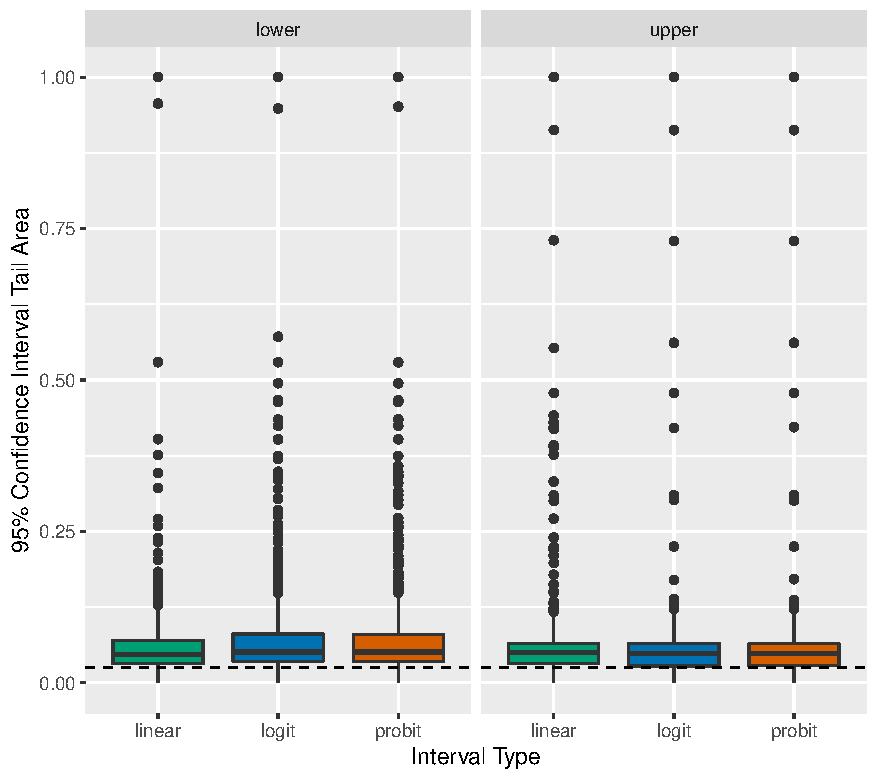
\includegraphics{intervalcomparison.pdf}

\footnotesize
Plotted values represent the ``non-coverage'' in each tail region outside the 95\% confidence interval. Overall the three types of intervals appear similar in their performance. The transformed intervals more often have higher rates of non-coverage in the lower tail than the upper. Since the intervals have similar performance, in the \texttt{pkpredict} package logit-transformed intervals are used for \mic interval computations to enforce the $[0,1]$ bounds.
\end{figure}


% % Other things to include in results?
% \begin{itemize}
% \item quantified posterior probability contained within approximate intervals for $logit^{-1}(h(log \theta_i))$ - maybe in methods
% \item quantified computing time % give brief summary how long it takes on average to compute each interval using sampling or approx
% \item note: make sure to uncomment line below and set up the bibtex doc
% %\item use ``plasmode'' simulation to assess quality of method across variety of individuals (PK heterogeneity in this pop); recent example of plasmode use in \cite{Franklin2014}; pioneered by \cite{Vaughan2009} % make sure this line runs - might be an issue w/ configuring bibtex document
% \end{itemize}




% \section{Package Contents}
%
% The primary function within the \texttt{pkm} package is the \texttt{pkm} function.


\section{Example}

Below we provide an example outlining how to implement this methodology using the \texttt{pkpredict} package. The minimum amount of information required to use the provided functions is the infusion schedule for a given patient of interest. All functions use data only associated with a single patient.

% \begin{itemize}
%   \item Generate ivt data frame
%   \item obtain raw mic estimate
%   \item fit pkm model
%   \item plot estimates
%   \item update the model and re-plot estimates
%   \item shiny app demo
% \end{itemize}

\begin{knitrout}
\definecolor{shadecolor}{rgb}{0.969, 0.969, 0.969}\color{fgcolor}\begin{kframe}
\begin{alltt}
\hlcom{# devtools::install_github("hlweeks/pkpredict")}
\hlkwd{library}\hlstd{(pkpredict)}
\end{alltt}
\end{kframe}
\end{knitrout}


\subsection{Sample infusion schedule and concentation data}
%Package functions: \texttt{ivt\_toList}

We have a vector of start times for five doses in hours since first infusion, and the duration of each dose. In this case, the duration is the same for each dose: half an hour. The rate of infusion is 6 g/h for all administered doses. Alternatively, the \texttt{ivt\_toList} function can take start and end dosing times rather than start times and duration.
\begin{knitrout}
\definecolor{shadecolor}{rgb}{0.969, 0.969, 0.969}\color{fgcolor}\begin{kframe}
\begin{alltt}
\hlcom{# Time in hours since first infusion}
\hlstd{start_times} \hlkwb{<-} \hlkwd{c}\hlstd{(}\hlnum{0}\hlstd{,} \hlnum{8}\hlstd{,} \hlnum{16}\hlstd{,} \hlnum{24}\hlstd{,} \hlnum{32}\hlstd{)}
\hlcom{# Duration of each infusion in hours}
\hlstd{duration} \hlkwb{<-} \hlnum{0.5}
\hlcom{# Rate in g/h}
\hlstd{rate_of_infusion} \hlkwb{<-} \hlkwd{rep}\hlstd{(}\hlnum{6}\hlstd{,} \hlnum{5}\hlstd{)}

\hlstd{ivt_d} \hlkwb{<-} \hlkwd{ivt_toList}\hlstd{(}\hlkwc{begin} \hlstd{= start_times,} \hlkwc{dur} \hlstd{= duration,} \hlkwc{rate} \hlstd{= rate_of_infusion)}
\end{alltt}
\end{kframe}
\end{knitrout}

% latex table generated in R 3.3.3 by xtable 1.8-2 package
% Tue Sep 26 10:31:42 2017
\begin{table}[ht]
\centering
\caption{Sample Infusion Schedule} 
\begin{tabular}{rrr}
  \hline
Begin (h) & End (h) & Infusion Rate (g/h) \\ 
  \hline
0.0 & 0.5 & 6.0 \\ 
  8.0 & 8.5 & 6.0 \\ 
  16.0 & 16.5 & 6.0 \\ 
  24.0 & 24.5 & 6.0 \\ 
  32.0 & 32.5 & 6.0 \\ 
   \hline
\end{tabular}
\end{table}


We also have sample data from three blood draws, with information on the concentration of piperacillin in the blood in $\mu$g/mL at the time at which the blood was drawn, again in hours since first infusion.
\begin{knitrout}
\definecolor{shadecolor}{rgb}{0.969, 0.969, 0.969}\color{fgcolor}\begin{kframe}
\begin{alltt}
\hlcom{# Time is in hours since first infusion}
\hlcom{# Concentration is in mcg/ml (or equivalently, mg/L)}
\hlstd{dat_d} \hlkwb{<-} \hlkwd{data.frame}\hlstd{(}\hlstr{"time"} \hlstd{=} \hlkwd{c}\hlstd{(}\hlnum{1}\hlstd{,} \hlnum{4}\hlstd{,} \hlnum{40}\hlstd{),}
                    \hlstr{"con"} \hlstd{=} \hlkwd{c}\hlstd{(}\hlnum{82.7}\hlstd{,} \hlnum{80.4}\hlstd{,} \hlnum{60}\hlstd{),}
                    \hlkwc{check.names} \hlstd{=} \hlnum{FALSE}\hlstd{)}
\end{alltt}
\end{kframe}
\end{knitrout}

% latex table generated in R 3.3.3 by xtable 1.8-2 package
% Tue Sep 26 10:31:43 2017
\begin{table}[ht]
\centering
\caption{Sample Data (observed from blood draws)} 
\begin{tabular}{rr}
  \hline
Time (h) & Concentration (mcg/mL) \\ 
  \hline
1.0 & 82.7 \\ 
  4.0 & 80.4 \\ 
  40.0 & 60.0 \\ 
   \hline
\end{tabular}
\end{table}



\subsection{MIC estimates}
%package functions: \texttt{mic_stat}

First, we obtain a prior estimate of target attainment based on the infusion schedule outlined above. By default, the \texttt{mic\_stat} function calculates the $fT > 4 \times MIC$, using a threshold of 64 $\mu$g/mL for piperacillin. The dosing window is assumed to end 12 hours after the end of the final infusion, and can be customized if desired.
\begin{knitrout}
\definecolor{shadecolor}{rgb}{0.969, 0.969, 0.969}\color{fgcolor}\begin{kframe}
\begin{alltt}
\hlcom{# Threshold is in mcg/mL (same scale as observed data)}
\hlcom{# By default, considering time through 12 hours after end of the final dose}

\hlcom{# Prior estimate}
\hlstd{prior_ft.mic} \hlkwb{<-} \hlkwd{mic_stat}\hlstd{(}\hlkwc{ivt} \hlstd{= ivt_d,} \hlkwc{th} \hlstd{=} \hlnum{64}\hlstd{)}
\hlstd{prior_ft.mic}
\end{alltt}
\begin{verbatim}
## $ftmic
## [1] 0.4782617
## 
## $conf.int
## [1] 0.09186105 0.89255457
## 
## attr(,"class")
## [1] "mic"  "list"
\end{verbatim}
\end{kframe}
\end{knitrout}

Without considering patient response from blood draws, the model estimates a patient on this infusion schedule will spend 47.8\% (95\% CI 9.2\% - 89.3\%) of their time above the desired threshold. This prior estimate of target attainment represents how we would expect a typical patient to respond to treatment over the course of this infusion schedule, in lieu of any blood concentration measurements. We can incorporate the observed blood draws and obtain an individualized estimate of target attainment based on the patient's data. By adding in concentration measurements from blood draws, we obtain posterior estimates.

\begin{knitrout}
\definecolor{shadecolor}{rgb}{0.969, 0.969, 0.969}\color{fgcolor}\begin{kframe}
\begin{alltt}
\hlcom{# Posterior estimate after observed measurements}
\hlstd{post_ft.mic} \hlkwb{<-} \hlkwd{mic_stat}\hlstd{(}\hlkwc{ivt} \hlstd{= ivt_d,} \hlkwc{dat} \hlstd{= dat_d,} \hlkwc{th} \hlstd{=} \hlnum{64}\hlstd{)}
\hlstd{post_ft.mic}
\end{alltt}
\begin{verbatim}
## $ftmic
## [1] 0.7352296
## 
## $conf.int
## [1] 0.4755578 0.8947764
## 
## attr(,"class")
## [1] "mic"  "list"
\end{verbatim}
\end{kframe}
\end{knitrout}


Our updated estimate of \mic is 73.5\% (95\% CI 47.6\% - 89.5\%). By default, the \texttt{mic_stat} function uses the Laplace approximation to calculate an approximate credible interval for target attainment. The user can also specify the argument \texttt{mcmc = TRUE} to use MCMC to obtain a more precise credible interval.


\subsection{PK Model}
%package functions: \texttt{pkm}

The \texttt{pkm} function fits a two-compartment model to obtain estimates of the concentation-time curve and \mic.

\begin{knitrout}
\definecolor{shadecolor}{rgb}{0.969, 0.969, 0.969}\color{fgcolor}\begin{kframe}
\begin{alltt}
\hlcom{# Fit the PK model}
\hlstd{pk.fit} \hlkwb{<-} \hlkwd{pkm}\hlstd{(}\hlkwc{formula} \hlstd{= con} \hlopt{~} \hlstd{time,} \hlkwc{data} \hlstd{= dat_d,}
              \hlkwc{ivt} \hlstd{= ivt_d,} \hlkwc{thres} \hlstd{=} \hlnum{64}\hlstd{)}
\hlstd{pk.fit}\hlopt{$}\hlstd{ftmic}
\end{alltt}
\begin{verbatim}
## $ftmic
## [1] 0.7352296
## 
## $conf.int
## [1] 0.4755578 0.8947764
## 
## attr(,"class")
## [1] "mic"  "list"
\end{verbatim}
\end{kframe}
\end{knitrout}

The model MIC statistic is exactly that produced by the \texttt{mic_stat} function.

Below we extract the predicted concentration values. The estimated concentration of drug in the bloodstream at the supplied start and end of infusion times, and (if applicable) the times associated with concentration measurements from the model.

%all.equal(pred.df$conc,  predict(pk.fit)[,"Concentration"])
%Update predict.pkm to provide confidence intervals rather than SE? Or keep as SE?

\begin{knitrout}
\definecolor{shadecolor}{rgb}{0.969, 0.969, 0.969}\color{fgcolor}\begin{kframe}
\begin{alltt}
\hlstd{pred.df} \hlkwb{<-} \hlstd{pk.fit}\hlopt{$}\hlstd{fitted.values}

\hlkwd{names}\hlstd{(pred.df)} \hlkwb{<-} \hlkwd{c}\hlstd{(}\hlstr{"Time Since First Infusion (h)"}\hlstd{,} \hlstr{"Concentration (mcg/mL)"}\hlstd{,} \hlstr{"Standard Error"}\hlstd{)}
\end{alltt}
\end{kframe}
\end{knitrout}

% latex table generated in R 3.3.3 by xtable 1.8-2 package
% Tue Sep 26 10:31:45 2017
\begin{table}[ht]
\centering
\caption{Predicted Values} 
\begin{tabular}{ccc}
  \hline
Time Since First Infusion (h) & Concentration (mcg/mL) & Standard Error \\ 
  \hline
0.00 & 0.20 & 0.11 \\ 
  0.50 & 97.34 & 0.11 \\ 
  1.00 & 91.58 & 0.10 \\ 
  4.00 & 63.51 & 0.08 \\ 
  8.00 & 38.99 & 0.10 \\ 
  8.50 & 134.03 & 0.09 \\ 
  16.00 & 53.68 & 0.13 \\ 
  16.50 & 147.85 & 0.08 \\ 
  24.00 & 59.22 & 0.14 \\ 
  24.50 & 153.07 & 0.08 \\ 
  32.00 & 61.32 & 0.15 \\ 
  32.50 & 155.03 & 0.08 \\ 
  40.00 & 62.11 & 0.16 \\ 
   \hline
\end{tabular}
\end{table}



Calling \texttt{plot} on the model object returns a visual representation of the patient's concentration-time curve for the administered drug.

\begin{figure}
\begin{knitrout}
\definecolor{shadecolor}{rgb}{0.969, 0.969, 0.969}\color{fgcolor}\begin{kframe}
\begin{alltt}
\hlkwd{plot}\hlstd{(pk.fit)}
\end{alltt}
\end{kframe}
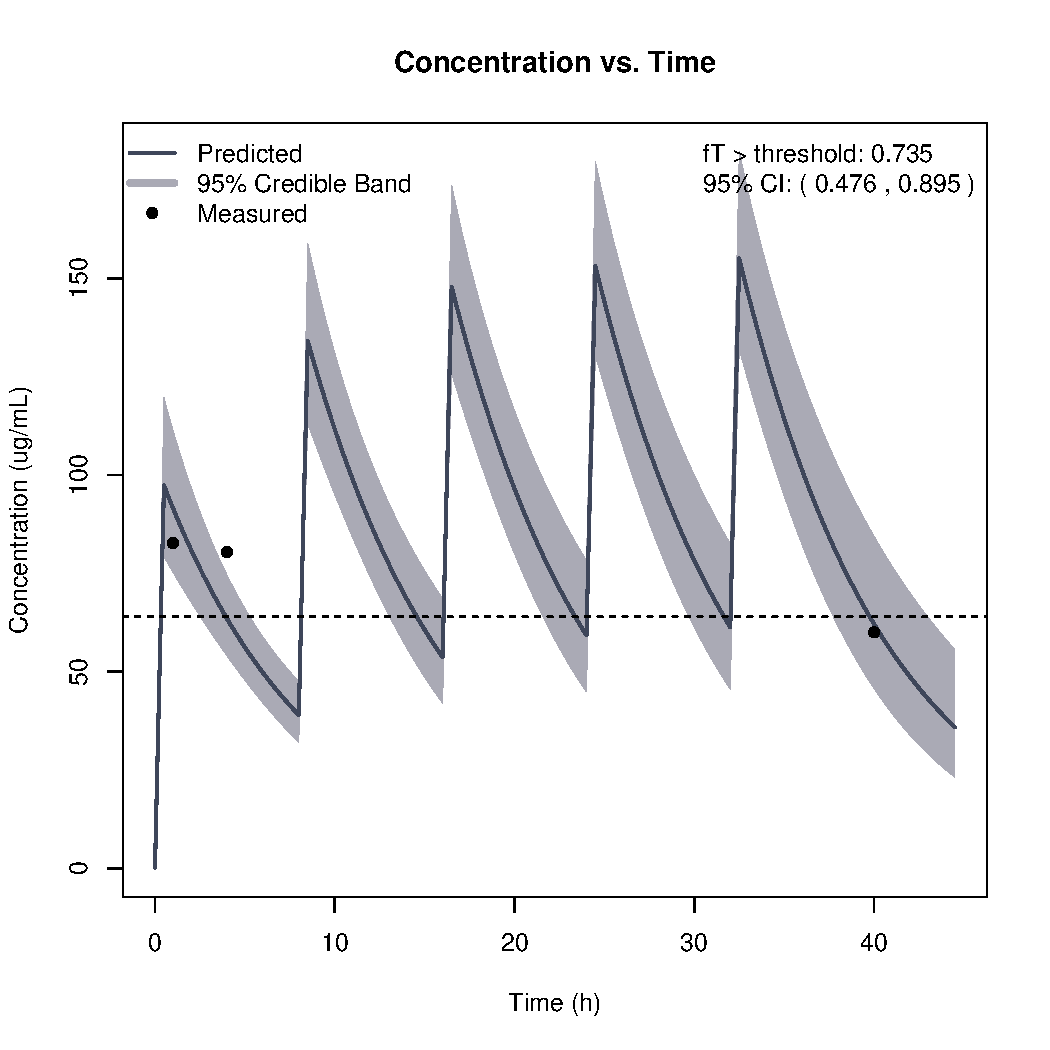
\includegraphics[width=\maxwidth]{figure/unnamed-chunk-15-1} 

\end{knitrout}
\end{figure}



\newpage

\subsection{Shiny GUI}

An interactive implementation of the methods presented here can be launched within the package by calling \texttt{shiny_pkm}. This function procudes a web application, created using the {\it shiny} package in R. In the application, users can enter information about a patient's infusion schedule and and concentration data collected from blood draws. By default, the application uses the infusion schedule in the example above. There is a checkbox option to allow for computation of the \mic credible interval using Markov chain Monte Carlo sampling for an exact interval. This method is more accurate, but takes much longer to perform.

\begin{knitrout}
\definecolor{shadecolor}{rgb}{0.969, 0.969, 0.969}\color{fgcolor}\begin{kframe}
\begin{alltt}
\hlkwd{shiny_pkm}\hlstd{()}
\end{alltt}
\end{kframe}
\end{knitrout}


\begin{figure}
\caption{Screenshot of Shiny application run using \texttt{shiny_pkm()}}

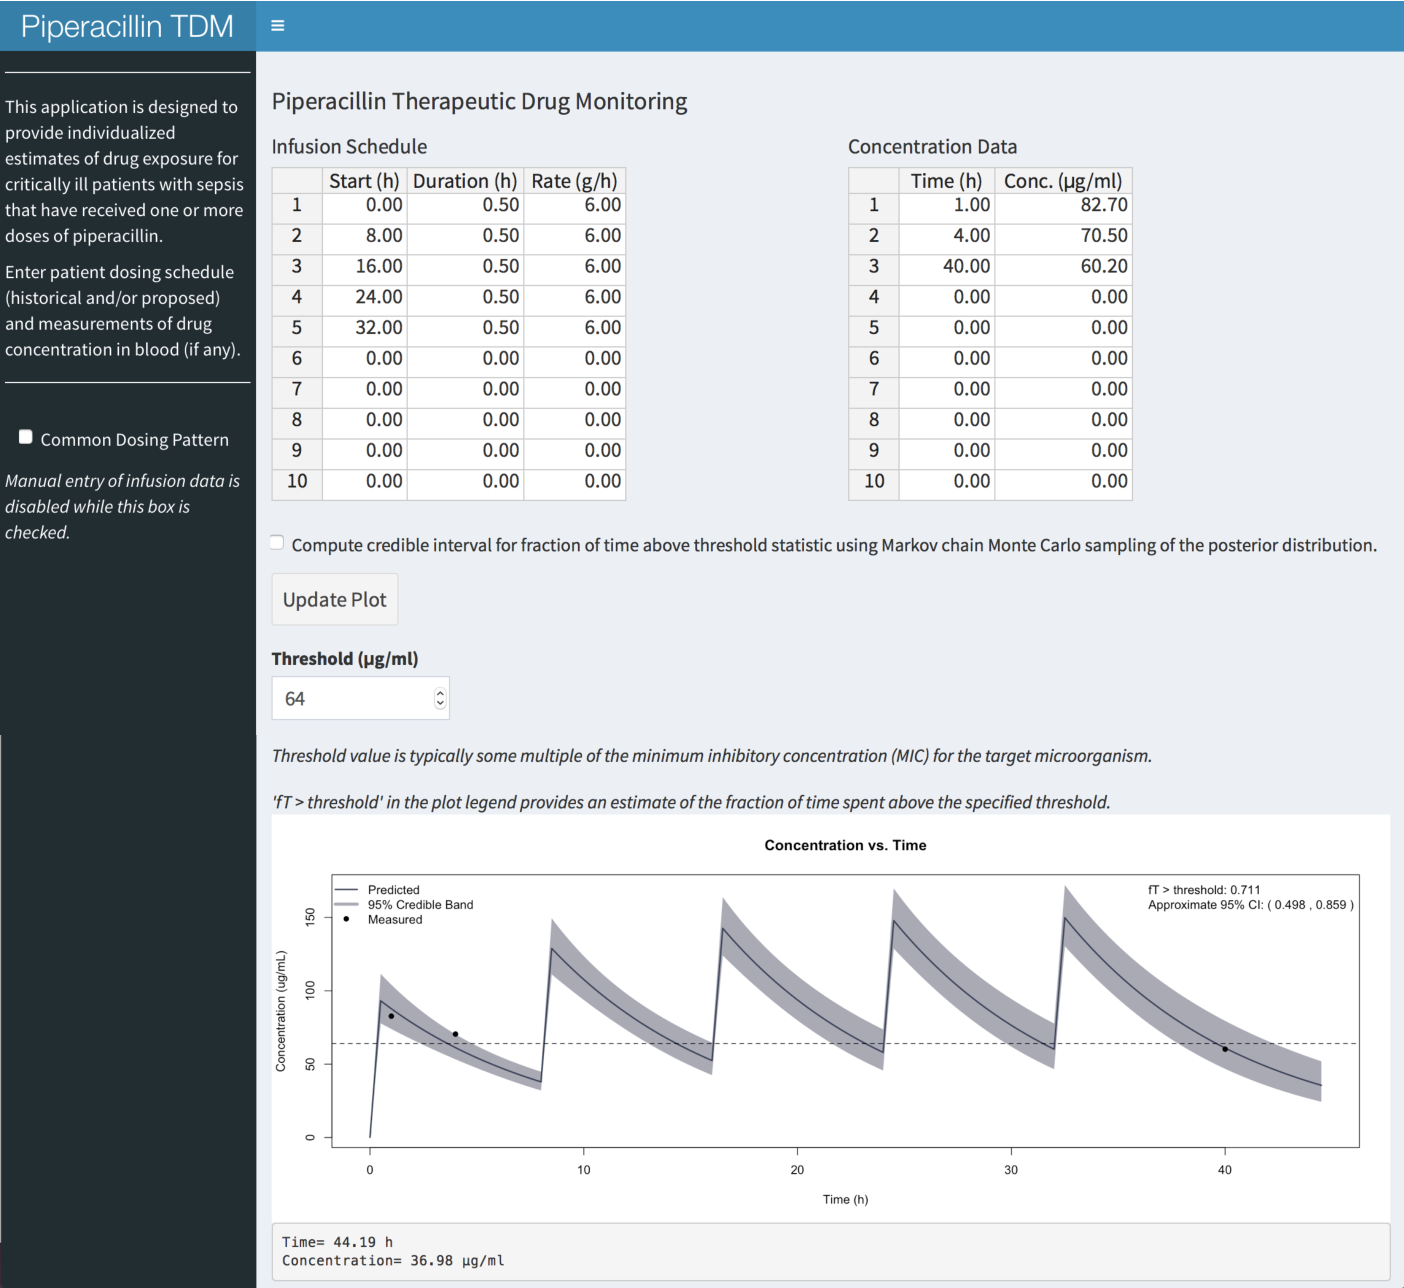
\includegraphics[scale=0.5]{appscreenshot.pdf}

\end{figure}






\section{Appendix: Prior hyperparameters for piperacillin among critically ill}
\begin{center}
\begin{table}
\begin{tabular}{lll} \hline
Parameter & Value \\ \hline
log($\mu_0$) & = (lv_1=3.223, lk_10=-1.650, lk_12 = -7, lk_21 = -7)\\
$\Sigma_0$ & $\sim$ 300 $\times$ $\begin{bmatrix} 0.00167 & -0.00128 & 0 & 0\\
                                -0.00128 & 0.00154 &      0 &      0 \\
                                       0 &       0 & .00015 &      0 \\
                                       0 &       0 &      0 & .00015)\end{bmatrix}$ \\ % log?
\hline
\end{tabular}
\caption{Prior hyperparameters for piperacillin in a population of hospitalized, critically ill patients.}\label{tab:hyp}
\end{table}
\end{center}



\end{document}
